\documentclass[table,dvipsnames]{beamer}
\mode<presentation>{
	\usetheme{Madrid}
	\setbeamercolor{title}{fg=Black,bg=Blue!15}
	\setbeamercolor{frametitle}{fg=Black,bg=Blue!15}
	\setbeamercolor{block title}{fg=Black,bg=Blue!15}
	\setbeamercolor{block}{fg=Black,bg=Blue!10}
}

\usepackage{default}
\usepackage{graphicx}
\usepackage{booktabs}
\usepackage{xcolor}
\usepackage{multirow}
\usepackage{minted}

\definecolor{LightGray}{gray}{0.9}

\title[STM32 Beginner Guide]{Pengenalan Multithreading dan Interfacing STM32}
\author{}
\institute[CodeDirect-FTITOS]{
	Achmadi ST MT\\
	\medskip
	\textit{}
}
\date{}

\begin{document}

	\section{Start}

	\begin{frame}
	\titlepage
	\end{frame}

	\begin{frame}
		\frametitle{G-Drive Resource}
		\begin{exampleblock}{}
			\begin{exampleblock}{}
			Seluruh file program,installer, dan sourcecode
			yang telah disiapkan dapat didownload di alamat:\\
			\end{exampleblock}
			
			\begin{exampleblock}{}
			\url{https://drive.google.com/open?id=16aN7ICZEpCad6L_2Q1hTNmetX-H0cCP7}
			\end{exampleblock}
		\end{exampleblock}
	\end{frame}

	\section{STM32}
	\subsection{Chip STM32}
	\begin{frame}
		\frametitle{Produk Chip STM32}
		\begin{exampleblock}{}
			Chip STM32 adalah microcontroller yang diproduksi ST Microelectronic.
		\end{exampleblock}

		\begin{exampleblock}{}
			Menggunakan arsitektur 32-bit ARM Cortex M0/M3/M4.
		\end{exampleblock}

		\begin{exampleblock}{}
			Standar Industri, tersedia tools dan compiler/toolchain untuk development.
		\end{exampleblock}
		\begin{center}
			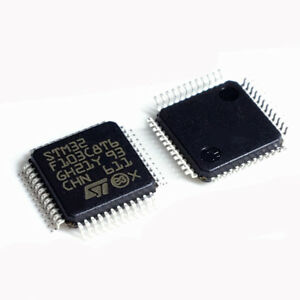
\includegraphics[width=150pt]{images/stm32f103c8}
		\end{center}
	\end{frame}

	\subsection{Board Discovery}
	\begin{frame}
		\frametitle{STM32 Discovery}
		\begin{exampleblock}{}
			ST menyediakan beberapa macam board untuk belajar pemula maupun pengembangan awal.
		\end{exampleblock}

		\begin{center}
			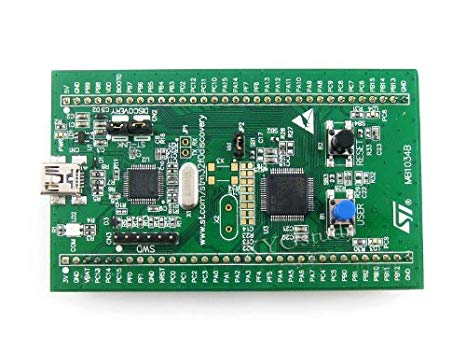
\includegraphics[width=150pt]{images/f0disco}
			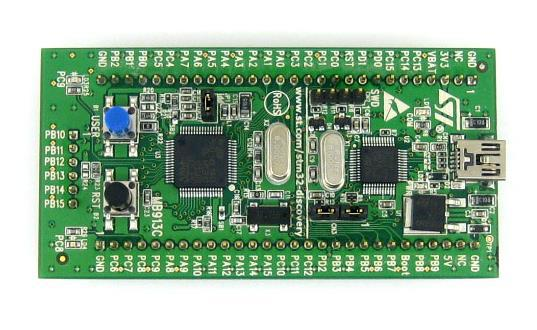
\includegraphics[width=150pt]{images/f1disco}
		\end{center}
	\end{frame}

	\begin{frame}
		\frametitle{STM32 Discovery}

		\begin{exampleblock}{}
			Tersedia board Discovery untuk seri STM32F0, STM32F1, STM32F2, STM32F3, dan STM32F4.
		\end{exampleblock}

		\begin{center}
			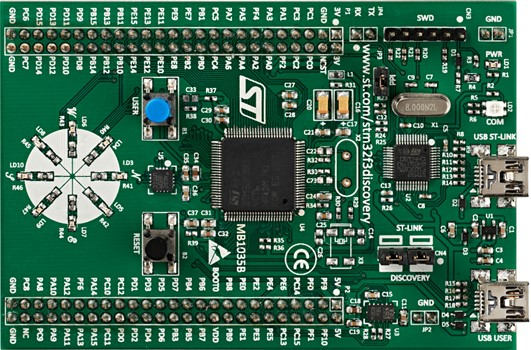
\includegraphics[width=125pt]{images/f3disco}
			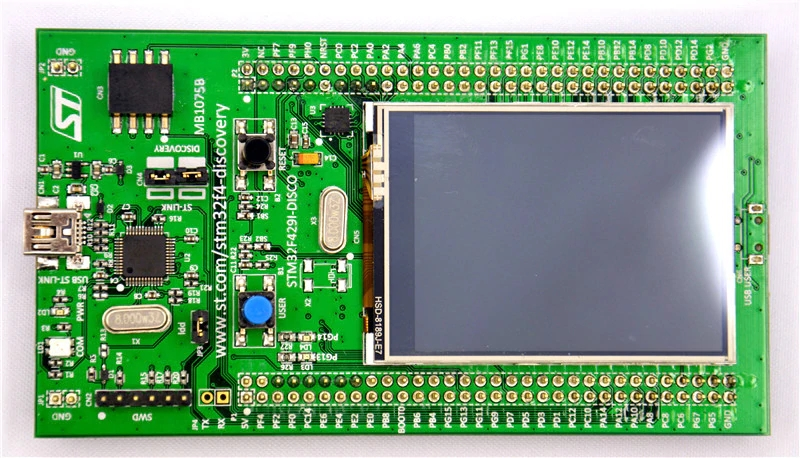
\includegraphics[width=150pt]{images/f4disco}
		\end{center}
	\end{frame}

	\subsection{Nucleo Discovery}
	\begin{frame}
		\frametitle{STM32 Nucleo}
		\begin{exampleblock}{}
			Selain Discovery, ST juga menyediakan board Nucleo yang memiliki pin-header layout
			kompatibel dengan Arduino.
		\end{exampleblock}

		\begin{center}
			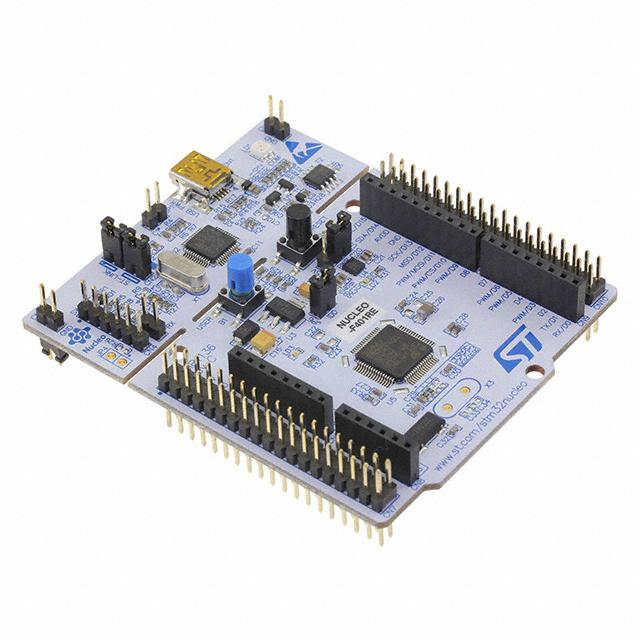
\includegraphics[width=200pt]{images/nucleo}
		\end{center}
	\end{frame}

	\subsection{Unofficial Board}
	\begin{frame}
		\frametitle{STM32 Unofficial Board}
		\begin{exampleblock}{}
			Selain Discovery dan Nucleo, tersedia juga board STM32 yang bukan dibuat oleh ST.
		\end{exampleblock}

		\begin{center}
			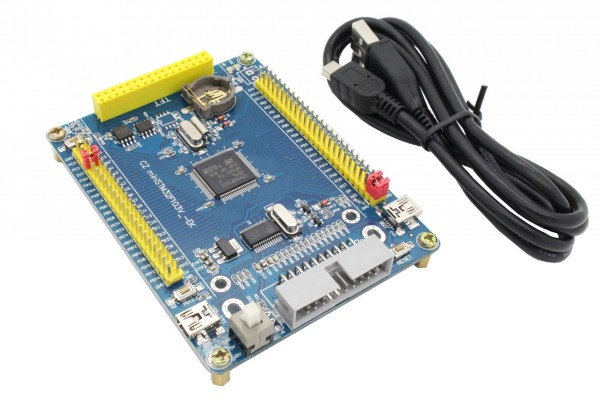
\includegraphics[width=150pt]{images/czmini}
			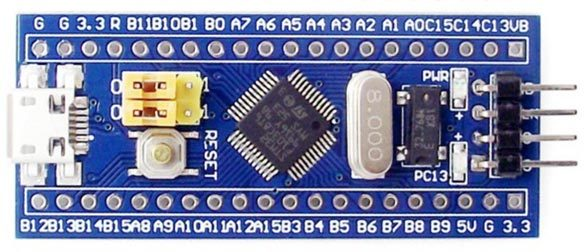
\includegraphics[width=150pt]{images/bluepill}
		\end{center}
	\end{frame}

	\section{Instalasi}
	\subsection{Driver}
	\begin{frame}
		\frametitle{Instalasi Driver}
		\begin{exampleblock}{}
			Install driver USB-TTL PL2303, ada di berkas \textbf{installer$\backslash$driver$\backslash$pl2303\_usb\_ttl.zip}
		\end{exampleblock}

		\begin{exampleblock}{}
			Untuk Windows 10 mungkin perlu update dan memilih versi driver secara manual dengan opsi
			\textit{Let me pick a list of available driver on my computer}.
		\end{exampleblock}

		\begin{exampleblock}{}
			Setelah instalasi driver PL2303, cek Device Manager untuk mengetahui nomor COM port
		\end{exampleblock}

		\begin{center}
			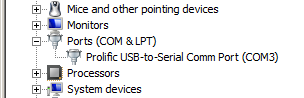
\includegraphics[width=175pt]{images/comport}
		\end{center}
	\end{frame}

	\subsection{Development Tools}
	\begin{frame}
		\frametitle{Compiler/Toolchain}
		\begin{exampleblock}{}
			\begin{itemize}
				\item Ekstrak file \textbf{STM32\_DevTools.zip} ke alamat semisal \textbf{C:$\backslash$}.
				\item Salin alamat folder binary compiler, semisal \textbf{C:$\backslash$STM32\_DevTools$\backslash$arm-gcc-suite$\backslash$bin}
				\item Masukkan alamatnya ke \textit{Environment Variabels}.
				\begin{itemize}
					\item Buka \textit{Computer} $\rightarrow$ \textit{Properties} $\rightarrow$ \textit{Advanced System Settings}
					\item Klik \textit{Environment Variables}
					\item Klik \textit{Path} yang ada dikolom \textit{System Variables}.
					\item Masukkan alamat tersebut (pisah dengan tanda koma).
				\end{itemize}
			\end{itemize}
		\end{exampleblock}

		\begin{center}
			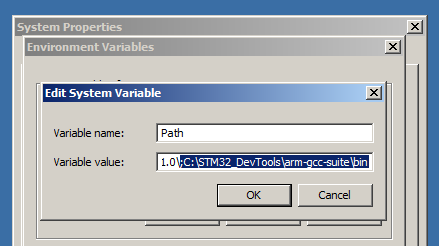
\includegraphics[width=150pt]{images/envar}
		\end{center}
	\end{frame}

	\begin{frame}
		\frametitle{Programmer Notepad}
		\begin{exampleblock}{}
			\begin{itemize}
				\item Buka Folder \textbf{STM32\_DevTools$\backslash$programmer-notepad}
				\item Jalankan program \textbf{programmer-notepad.exe} dengan \textit{Run as Administrator}.
				\item Programmer Notepad digunakan untuk kompilasi \textit{sourcecode} ke binary yang siap didownload ke STM32.
			\end{itemize}
		\end{exampleblock}

		\begin{center}
			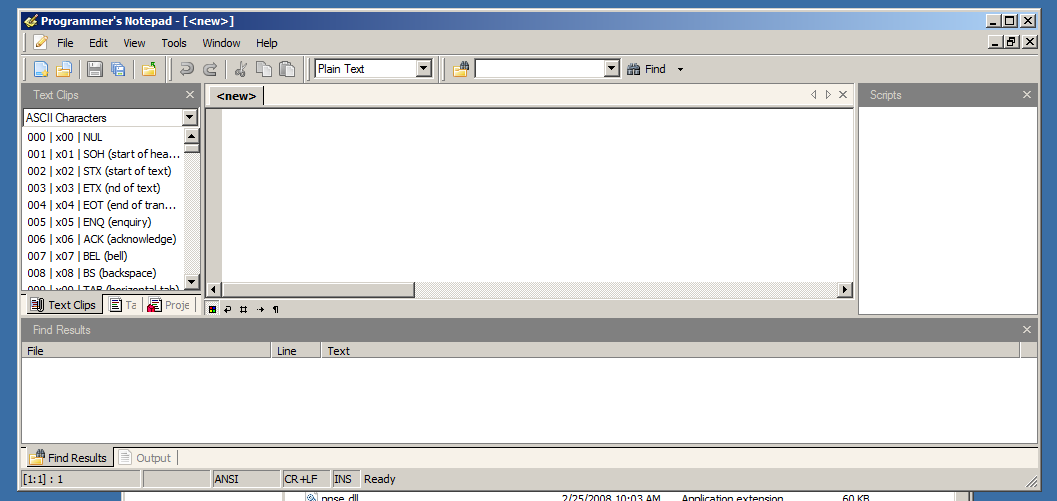
\includegraphics[width=250pt]{images/pn}
		\end{center}
	\end{frame}

	\begin{frame}
	\frametitle{Tes Example}
	\begin{exampleblock}{}
		\begin{itemize}
			\item Ekstrak \textbf{ChibiOS\_STM32.zip}.
			\item Buka dengan Programmer Notepad berkas Makefile di folder \textbf{ChibiOS\_STM32$\backslash$example$\backslash$BLUEPILL-BLINK}.
			\item Untuk kompilasi, klik \textit{Tools} $\rightarrow$ \textit{Make All}
		\end{itemize}
	\end{exampleblock}

	\begin{center}
		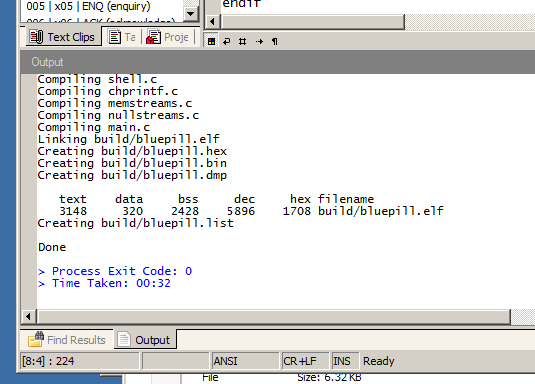
\includegraphics[width=200pt]{images/compile}
	\end{center}
	\end{frame}

	\subsection{Flashloader}
	\begin{frame}
	\frametitle{STM32 bootloader}
		\begin{exampleblock}{}
			Saat running $\rightarrow$ Main Flash Memory
		\end{exampleblock}
		\begin{exampleblock}{}
			Saat programming $\rightarrow$ System Memory
		\end{exampleblock}

		\begin{center}
			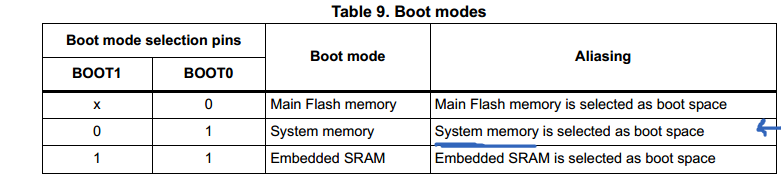
\includegraphics[width=300pt]{images/bootloader}
		\end{center}
	\end{frame}

	\begin{frame}
		\frametitle{UART Line}
		\begin{exampleblock}{}
			Sambungan STM32 ke PL2303 (USB-Serial TTL)
			\begin{itemize}
				\item STM32 5v $\rightarrow$ PL2303 5v
				\item STM32 GND $\rightarrow$ PL2303 GND
				\item STM32 TX (PA9) $\rightarrow$ PL2303 RX
				\item STM32 RX (PA10) $\rightarrow$ PL2303 TX
			\end{itemize}
		\end{exampleblock}

		\begin{exampleblock}{}
			\textbf{WARNING}: Jangan sambungkan STM32 3.3v pin ke 5v.
			Maximal toleransi tegangan VDD STM32 hanya sampai 3.6 volt.
		\end{exampleblock}
	\end{frame}

	\begin{frame}
		\frametitle{Aktivasi bootloader}
		\begin{exampleblock}{}
			Aktifkan bootloader untuk untuk masuk mode programming.
			\begin{itemize}
				\item pindahkan jumper \textbf{boot0} ke logic 1.
				\item jumper \textbf{boot1} tetap di logic 0.
				\item tekan reset
			\end{itemize}
		\end{exampleblock}

		\begin{center}
			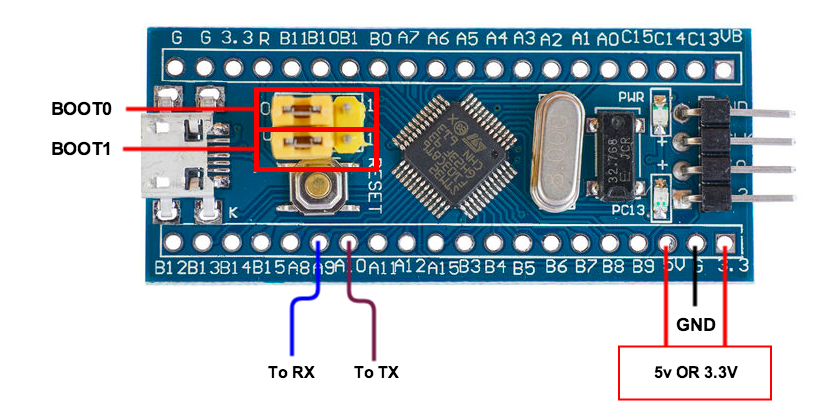
\includegraphics[width=300pt]{images/flashing}
		\end{center}
	\end{frame}

	\subsection{Demonstrator}
	\begin{frame}
		\frametitle{Installasi Demonstrator}
		\begin{exampleblock}{}
			Demonstrator adalah program sederhana untuk download binary ke chip STM32 dengan bantuan internal bootloader via UART-Line.
			\begin{itemize}
				\item Install program Demonstrator yang ada di \textbf{installer$\backslash$tools$\backslash$stm32\_flasher.zip}
				\item Jalankan Demonstator GUI dari menu dengan \textit{Run as Administrator}.
				\item Pastikan nomor COM port sesuai dengan nomor serial port PL2302 di Device Manager.
			\end{itemize}
		\end{exampleblock}

		\begin{center}
			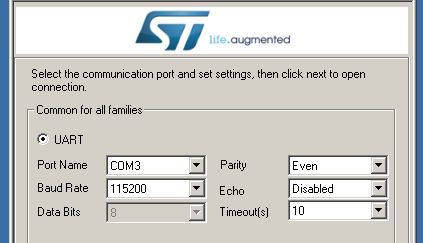
\includegraphics[width=150pt]{images/demons}
		\end{center}
	\end{frame}

	\subsection{Downloading}
	\begin{frame}
		\frametitle{Next}
		\begin{exampleblock}{}
			Klik \textit{Next}. Jika ada pesan error, cek wiring, kondisi jumper boot, dan tekan reset lagi.
		\end{exampleblock}
		\begin{center}
			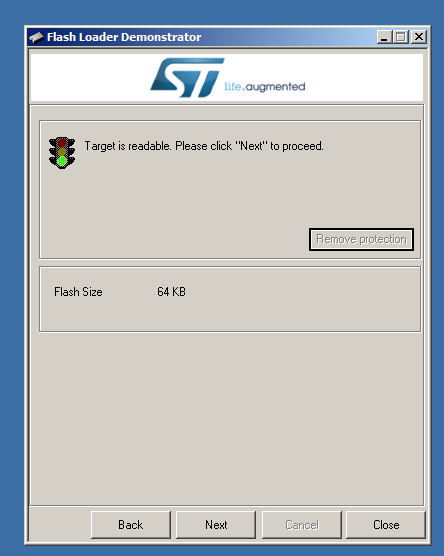
\includegraphics[width=150pt]{images/demons1}
			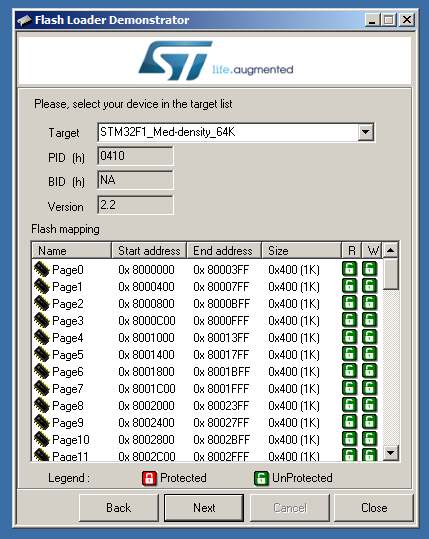
\includegraphics[width=150pt]{images/demons2}
		\end{center}
	\end{frame}

	\begin{frame}
		\frametitle{Download binary}
		\begin{exampleblock}{}
			\begin{itemize}
				\item pilih \textit{Download to Device}
				\item isi alamat file yang akan di download:
				\begin{itemize}
					\item Klik browser (simbol tiga titik) disebelah address bar
					\item Di open file dialog, pilih tipe file \textbf{*.bin} atau \textbf{*.hex}
					\item Cari file yanga akan didownload ke chip, sebagai contoh disini:\\
					\textbf{ChibiOS\_STM32$\backslash$example$\backslash$BLUEPILL-BLINK$\backslash$build$\backslash$bluepill.bin}.
				\end{itemize}
				\item Klik \textit{Global Erase}.
				\item Centang \textit{Verify after download}.
			\end{itemize}
		\end{exampleblock}
		\begin{center}
			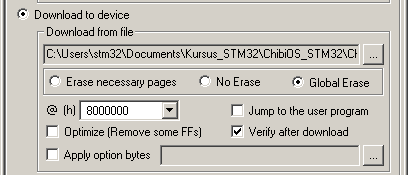
\includegraphics[width=200pt]{images/demons3}
		\end{center}
	\end{frame}

	\begin{frame}
		\frametitle{Download Success}
		\begin{exampleblock}{}
			Tunggu proses Downloading selesai dan sukses.
			Program Demonstrator bisa di \textit{Close}.
		\end{exampleblock}
		\begin{center}
			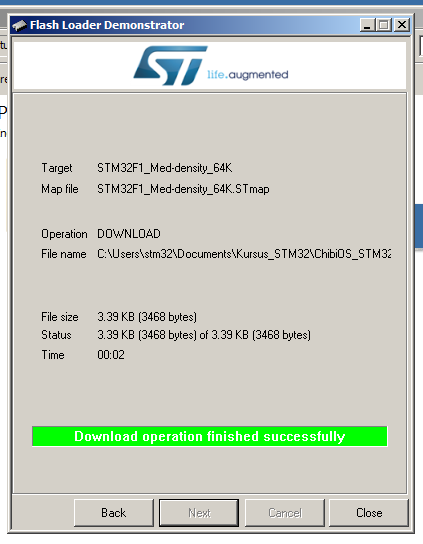
\includegraphics[width=150pt]{images/demons4}
		\end{center}
	\end{frame}

	\begin{frame}
		\frametitle{Aktivasi Main Program}
		\begin{exampleblock}{}
			Aktivasi Main program untuk untuk masuk mode running.
			\begin{itemize}
				\item pindahkan jumper \textbf{boot0} ke logic 0.
				\item jumper \textbf{boot1} tetap di logic 0.
				\item tekan reset
			\end{itemize}
		\end{exampleblock}

		\begin{center}
			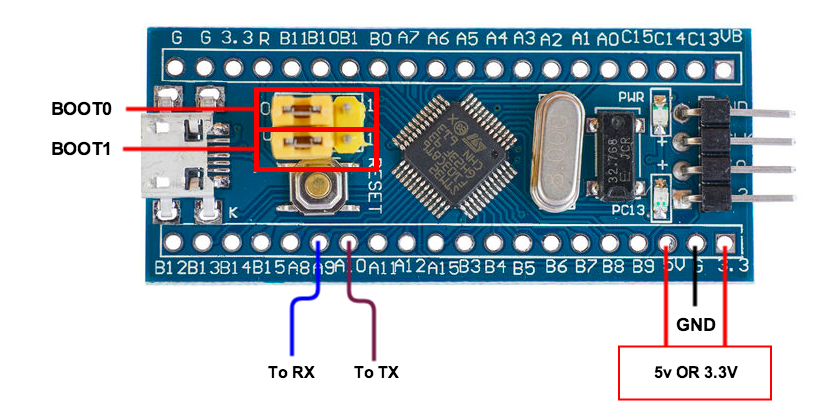
\includegraphics[width=300pt]{images/flashing}
		\end{center}
	\end{frame}

	\section{ChibiOS}
	\subsection{Overview}
	\begin{frame}
		\frametitle{ChibiOS}
		\begin{exampleblock}{}
			ChibiOS/RT buatan Giovanni D. Sirrio, adalah pustaka (library) yang berfungsi sebagai middleware untuk menjembatani program/aplikasi yang dibuat programmer
			dan sistem \textit{low-level} untuk banyak \textit{embedded-device} berbasis ARM (STM32 adalah salah satunya).
		\end{exampleblock}

		\begin{exampleblock}{}
			ChibiOS/RT menyediakan antara lain:
			\begin{itemize}
				\item HAL (Hardware Abstraction Layer) sebagai source-based driver.
				\item Scheduling untuk multitask CPU sehingga bisa dilakukan multithreading.
				\item Binding ke library lain semisal:
				\begin{itemize}
					\item FatFs untuk emulasi filesystem FAT16/FAT32.
					\item LwIP untuk emulasi network UDP/TCP IP.
					\item uGFX untuk driver spesifik LCD grafik dan TFT touchscreen.
				\end{itemize}
			\end{itemize}
		\end{exampleblock}
	\end{frame}

	\begin{frame}
		\frametitle{ChibiOS}
		\begin{exampleblock}{}
			ChibiOS/RT untuk penggunaan gratis bersifat open-source sesuai lisensi GPLv3.
		\end{exampleblock}

		\begin{exampleblock}{}
			\textbf{Catatan}: lisensi open-source pada hakikatnya hanya memiliki aturan sebagai berikut:
			\begin{itemize}
				\item Suatu sourcecode dan turunannya harus memiliki lisensi yang sama.
				\item Pengembang harus memberikan akses sourcecode yang dibuat, baik dengan gratis atau berbayar.
				\item Pengembang berhak akses modifikasi (patch) dari pengembang lain, baik dengan gratis atau berbayar.
				\item Sourcecode maupun binary-nya boleh disebarkan dengan gratis atau dijual dengan harga sesuka hati.
			\end{itemize}
		\end{exampleblock}
	\end{frame}

	\begin{frame}
		\frametitle{ChibiOS}
		\begin{exampleblock}{}
			Paket ChibiOS/RT dapat didownload di alamat\\
			\url{http://chibios.org/dokuwiki/doku.php?id=chibios:downloads:start}.
		\end{exampleblock}

		\begin{exampleblock}{}
			\textbf{Catatan}: Untuk versi, disarankan mendownload dan menggunakan versi 2.x atau 3.x.
		\end{exampleblock}

		\begin{exampleblock}{}
			Alternatif middleware lain untuk STM32:
			\begin{itemize}
				\item \textbf{Std\_Periph}, pustaka HAL/Driver resmi dari ST. Tidak menyediakan scheduling multitask.
				\item \textbf{Free-RTOS}, pustaka scheduling multitask tanpa HAL/Driver. Sering dikombinasi dengan pustaka Std\_Periph.
			\end{itemize}
		\end{exampleblock}
	\end{frame}

	\subsection{Requierement}
	\begin{frame}
		\frametitle{Basic Programming}
		\begin{exampleblock}{}
			Untuk pemrograman dengan ChibiOS, hanya dibutuhkan toolchain arm-gcc dan paket ChibiOS.
		\end{exampleblock}

		\begin{exampleblock}{}
			Sourcecode minimal yang dibutuhkan:
			\begin{itemize}
				\item \textbf{chconf.h}. Berisi definisi dan pengaturan untuk scheduling multitask.
				Umumnya dibiarkan default.
				\item \textbf{halconf.h}. Berisi definisi dan pengaturan untuk driver yang masih hardware/chip independen.
				Perlu penyesuaian sesuai kebutuhan.
				\item \textbf{mcuconf.h}. Berisi definisi dan pengaturan untuk driver yang bergantung tipe/seri hardware/chip.
				Perlu penyesuaian sesuai kebutuhan dan mengacu kepada halconf.h.
				\item \textbf{main.c}. Minimal implementasi dan referensi untuk semua rutin yang dibutuhkan.
				\item \textbf{Makefile}. Berisi instruksi kompilasi, alamat ChibiOS beserta detil komponen, dan tambahan deklarasi/definisi.
			\end{itemize}
		\end{exampleblock}
	\end{frame}

	\subsection{Minimal main.c}
	\begin{frame}[fragile]
		\frametitle{Example}
		\begin{exampleblock}{}
			\begin{minted}[frame=lines,framesep=2mm,fontsize=\tiny,bgcolor=LightGray]{c}
#include "ch.h"
#include "hal.h"

int main(void) {

	halInit();
	chSysInit();

	while(true){
		chThdSleepMilliseconds(100);
	}
}
			\end{minted}
		\end{exampleblock}

		\begin{exampleblock}{}
			\textbf{Catatan:} Untuk setiap \textit{infinite-loop} atau \textit{while(true){}},
			wajib diberi delay minimal 1 microsecond untuk menghindari perilaku thread yang balapan dan menimbulkan crash/hunk.
		\end{exampleblock}
	\end{frame}

	\begin{frame}[fragile]
		\frametitle{Example dengan 2 thread}
		\begin{exampleblock}{}
			\begin{minted}[frame=lines,framesep=2mm,fontsize=\tiny,bgcolor=LightGray]{c}
#include "ch.h"
#include "hal.h"

static THD_WORKING_AREA(waThread, 128);
static THD_FUNCTION(thdThread, arg) {
	(void)arg;

	while (true) {
		chThdSleepMilliseconds(100);
	}
}

int main(void) {

	halInit();
	chSysInit();

	chThdCreateStatic(waThread, sizeof(waThread), NORMALPRIO, thdThread, NULL);

	while(true){
		chThdSleepMilliseconds(100);
	}
}
			\end{minted}
		\end{exampleblock}
	\end{frame}

		\begin{frame}[fragile]
		\frametitle{Example dengan 2 thread dan LED}
		\begin{exampleblock}{}
			\begin{minted}[frame=lines,framesep=2mm,fontsize=\tiny,bgcolor=LightGray]{c}
#include "ch.h"
#include "hal.h"

static THD_WORKING_AREA(waThread, 128);
static THD_FUNCTION(thdThread, arg) {
	(void)arg;

	while (true) {
		palTogglePad(GPIOC,13);
		chThdSleepMilliseconds(100);
	}
}

int main(void) {

	halInit();
	chSysInit();

	palSetPadMode(GPIOC,13,PAL_MODE_OUTPUT_PUSHPULL);
	chThdCreateStatic(waThread, sizeof(waThread), NORMALPRIO, thdThread, NULL);

	while(true){
		chThdSleepMilliseconds(100);
	}
}
			\end{minted}
		\end{exampleblock}
	\end{frame}

	\subsection{Hardware Abstraction}
	\begin{frame}
		\frametitle{Definisi HAL}
		\begin{exampleblock}{}
			Hardware Abstraction Layer adalah metode penulisan fungsi dalam suatu pustaka, dimana fungsi tersebut \textit{portable}
			dan dapat dipanggil ulang pada platform yang berbeda
		\end{exampleblock}

		\begin{exampleblock}{}
			Dalam pemrograman \textit{low-level} dan \textit{mid-level}, metode ini memudahkan programmer untuk tidak perlu
			menghafal alamat \textit{register} untuk instruksi maupun properti.
		\end{exampleblock}

		\begin{exampleblock}{}
			Beberapa contoh pustaka hardware abstraksi:
			\begin{itemize}
				\item Arduino
				\item ChibiOS
				\item STD\_Periph
				\item OpenCM3
			\end{itemize}
		\end{exampleblock}
	\end{frame}

	\begin{frame}[fragile]
		\frametitle{Komparasi Metode}
		\begin{exampleblock}{}
			Akses STM32 GPIO Register
			\begin{minted}[frame=lines,framesep=2mm,fontsize=\tiny,bgcolor=LightGray]{c}
RCC->APB2ENR = 0x0000000C;
GPIOC->CRH |= 0x00100000;
GPIOC->ODR |= 0x00000001;
			\end{minted}
		\end{exampleblock}

		\begin{exampleblock}{}
			Pengaturan di halconf.h dan implementasi di main.c
			\begin{exampleblock}{}
				\begin{minted}[frame=lines,framesep=2mm,fontsize=\tiny,bgcolor=LightGray]{c}
#define HAL_USE_PAL                 TRUE
				\end{minted}
			\end{exampleblock}

			\begin{exampleblock}{}
				\begin{minted}[frame=lines,framesep=2mm,fontsize=\tiny,bgcolor=LightGray]{c}
palSetPadMode(GPIOC,13,PAL_MODE_OUTPUT_PUSHPULL);
palSetPad(GPIOC,13);
				\end{minted}
			\end{exampleblock}
		\end{exampleblock}
	\end{frame}

	\subsection{New Example}
	\begin{frame}[fragile]
		\frametitle{New LED Example}
		\begin{exampleblock}{}
			Buat dua level folder dalam folder paket \textbf{ChibiOS\_STM32}:\\
			contoh \textbf{ChibiOS\_STM32$\backslash$contoh$\backslash$led}
		\end{exampleblock}

		\begin{exampleblock}{}
			Salin \textbf{chconf.h} dari contoh di:
			\textbf{ChibiOS\_STM32$\backslash$example$\backslash$BLUEPILL-LED}\\
			(Default pengaturan sudah cukup).
		\end{exampleblock}

		\begin{exampleblock}{}
			Salin \textbf{halconf.h} dari folder contoh yang sama sebelumnya.\\
			Cek fitur semisal PAL (Port Abstraction Layer) apakah sudah aktif.
			\begin{minted}[frame=lines,framesep=2mm,fontsize=\tiny,bgcolor=LightGray]{c}
#define HAL_USE_PAL                 TRUE
			\end{minted}
		\end{exampleblock}
	\end{frame}

	\begin{frame}
		\frametitle{New LED Example}
		\begin{exampleblock}{}
			Salin \textbf{mcuconf.h} dari folder contoh yang sama sebelumnya.\\
			Cek pengaturan clock, CPU frequency, dan peripheral apakah sudah sesuai kebutuhan dan pengaturan \textbf{halconf.h}.\\
			Jika tidak ada kebutuhan spesifik, default pengaturan sudah cukup.
		\end{exampleblock}

		\begin{exampleblock}{}
			Salin \textbf{main.c} dari folder contoh yang sama sebelumnya.\\
			Seluruh implementasi dapat dimulai dipanggil disini.
		\end{exampleblock}

		\begin{exampleblock}{}
			Salin \textbf{Makefile} dari folder contoh yang sama sebelumnya.\\
			Pastikan alamat paket ChibiOS, detil pustaka, dan semua file yang akan dikompilasi sudah benar.
		\end{exampleblock}

		\begin{exampleblock}{}
			Buka \textbf{Makefile} di Programmer Notepad dan \textbf{Make All} untuk kompilasi source ke binary.
		\end{exampleblock}
	\end{frame}

	\section{Serial Interface}

	\subsection{Overview}
	\begin{frame}
		\frametitle{Definisi Serial Communication}
		\begin{exampleblock}{}
			Serial Interface adalah protokol komunikasi yang paling umum digunakan.
			Salah satu protokol serial yang sangat umum digunakan adalah UART (Universal Asychronous Receiver-Transmitter).
		\end{exampleblock}

		\begin{exampleblock}{}
			Protokol UART hanya (minimal) membutuhkan RX, TX, dan GND.\\
			Jalur RX-TX bersilangan dan tidak ada hirarki Master-Slave.
		\end{exampleblock}

		\begin{exampleblock}{}
			Dalam penggunaan IoT, chip STM32 dapat dikomunikasikan dengan:
			\begin{itemize}
				\item Komputer melalui USB-TTL seperti PL2303, FT232RL, CH340X, dst.
				\item Emulasi protokol seperti Bluetooth HC05, UDP/TCP Wiznet, dst.
				\item Miniserver seperti NodeMCU, ESP8622, dst
				\item Microcomputer seperti RaspberryPi, Beaglebone, dst
				\item Microcontroller seperti Arduino/ATMega, PICF, dst
				\item Industrial Platform (via ModBUS/RS-485) seperti PLC, SCADA, dst.
			\end{itemize}
		\end{exampleblock}
	\end{frame}

	\begin{frame}
		\frametitle{Virtual Terminal}
		\begin{exampleblock}{}
			Virtual Terminal adalah program untuk interfacing serial terminal pada komputer/laptop.
		\end{exampleblock}

		\begin{exampleblock}{}
			Program ini tersedia di \textbf{STM32\_DevTools$\backslash$serial-terminal$\backslash$terminal-hercules.exe}.
			\begin{itemize}
				\item Jalankan dengan \textit{Run as Administrator}.
				\item Jika muncul konfirmasi unblock firewall, pilih \textit{Allow access}.
				\item Pilih tab Serial.
				\item Cek Device Manager untuk mengetahui nomor COM port.
				\item Pilih BaudRate sesuai program di STM32.
				\item Klik \textit{Open} untuk memulai akses protokol serial.
				\item Klik \textit{Close} untuk mengakhiri akses protokol serial.
			\end{itemize}
		\end{exampleblock}
	\end{frame}

	\begin{frame}
		\frametitle{Virtual Terminal}
		\begin{exampleblock}{}
			\begin{center}
				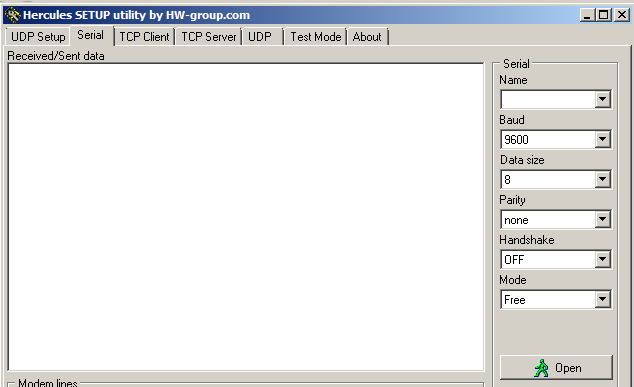
\includegraphics[width=300pt]{images/serterm}
			\end{center}
		\end{exampleblock}
	\end{frame}

	\subsection{Example UART}
	\begin{frame}[fragile]
		\frametitle{Simple UART}
		\begin{exampleblock}{}
			Salin BLUEPILL-LED sebagai basis untuk contoh ini.
		\end{exampleblock}

		\begin{exampleblock}{}
			Untuk \textbf{chconf.h} cukup gunakan default.
		\end{exampleblock}

		\begin{exampleblock}{}
			Untuk \textbf{halconf.h}, aktifkan SERIAL.
			\begin{minted}[frame=lines,framesep=2mm,fontsize=\tiny,bgcolor=LightGray]{c}
#define HAL_USE_SERIAL              TRUE
			\end{minted}
		\end{exampleblock}

		\begin{exampleblock}{}
			Untuk \textbf{mcuconf.h}, aktifkan SERIAL USART1.
			\begin{minted}[frame=lines,framesep=2mm,fontsize=\tiny,bgcolor=LightGray]{c}
#define STM32_SERIAL_USE_USART1             TRUE
			\end{minted}
		\end{exampleblock}
	\end{frame}

	\begin{frame}[fragile]
		\frametitle{Simple UART}
		\begin{exampleblock}{}
			Untuk main.c, tambahkan library string/char standard out.
			\begin{minted}[frame=lines,framesep=2mm,fontsize=\tiny,bgcolor=LightGray]{c}
#include "chprintf.h"
			\end{minted}
		\end{exampleblock}

		\begin{exampleblock}{}
			Tetap di \textbf{main.c}, aktifkan tambahkan fungsi start SERIAL.
			\begin{minted}[frame=lines,framesep=2mm,fontsize=\tiny,bgcolor=LightGray]{c}
palSetPadMode(GPIOA,9,PAL_MODE_STM32_ALTERNATE_PUSHPULL); //TX
palSetPadMode(GPIOA,10,PAL_MODE_INPUT); //RX
sdStart(&SD1,NULL);
			\end{minted}
		\end{exampleblock}

		\begin{exampleblock}{}
			Selanjutnya untuk infinite-loop di main.c, tambahkan fungsi menulis string ke serial UART-1.
			\begin{minted}[frame=lines,framesep=2mm,fontsize=\tiny,bgcolor=LightGray]{c}
chprintf((BaseSequentialStream *)&SD1,"Test Serial OK\n");
			\end{minted}
		\end{exampleblock}
	\end{frame}

	\begin{frame}
		\frametitle{Simple UART}
		\begin{exampleblock}{}
			\begin{center}
				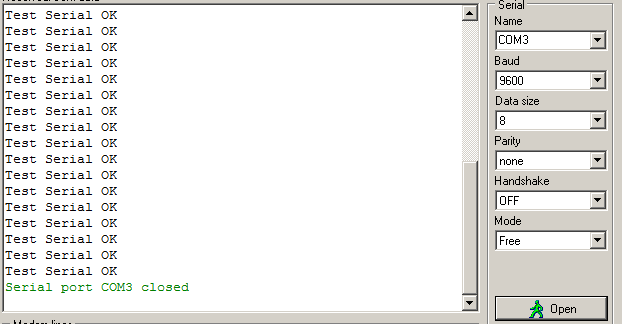
\includegraphics[width=250pt]{images/uart}
			\end{center}
		\end{exampleblock}
	\end{frame}

	\subsection{Example Shell}
	\begin{frame}
		\frametitle{Simple Shell}
		\begin{exampleblock}{}
			Untuk interaktif shell, berikut contoh yang telah disediakan:
			\begin{itemize}
				\item Buka \textbf{ChibiOS\_STM32$\backslash$example$\backslash$BLUEPILL-SHELL}.
				\item Buka \textbf{Makefile} dengan Programmer-Notepad dan \textbf{Make-All} untuk kompilasi.
				\item Download binary ke chip STM32.
				\item Setelah STM32 masuk mode running, akses serial dengan Virtual Terminal.
				\item Ketik "info" tanpa tanda petik ke Serial Terminal.
				\item Ketik "test" tanpa tanda petik ke Serial Terminal.
				\item Ketik "help" tanpa tanda petik ke Serial Terminal.
			\end{itemize}
		\end{exampleblock}
	\end{frame}

	\begin{frame}
		\frametitle{Simple Shell}
		\begin{exampleblock}{}
			\begin{center}
				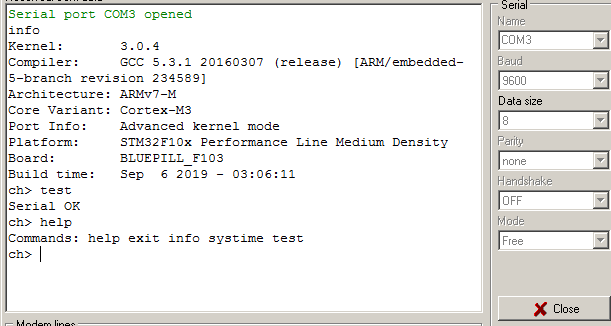
\includegraphics[width=250pt]{images/shell}
			\end{center}
		\end{exampleblock}
	\end{frame}

	\section{Komparasi Arduino/ATMega}

	\subsection{Multitask}
	\begin{frame}[fragile]
		\frametitle{Arduino UART}
		\begin{exampleblock}{}
			Example untuk LED dan Serial yang umum:
			\begin{minted}[frame=lines,framesep=2mm,fontsize=\tiny,bgcolor=LightGray]{c}
String kata;

void setup() {
	pinMode(LED_BUILTIN, OUTPUT);
	Serial.begin(9600);
}

void loop() {
	while(Serial.available()) {
		kata = Serial.readString();
		if(kata == "test"){
			Serial.println("Serial OK");
		}
	}

	digitalWrite(LED_BUILTIN, HIGH);
	delay(500);
	digitalWrite(LED_BUILTIN, LOW);
	delay(500);
}
			\end{minted}
		\end{exampleblock}
	\end{frame}

	\begin{frame}
		\frametitle{Arduino UART}
		\begin{exampleblock}{}
			Arduino LED dan Serial
			\begin{itemize}
				\item Setelah Arduino diprogram, LED akan berkedip.
				\item Jalankan virtual terminal dan akses serial port.
				\item Ketikan huruf/angka acak ke serial terminal.
				\item Saat menerima data karakter, LED akan berhenti berkedip.
				\item Proses main infinite-loop berhenti saat proses masuknya data karakter.
			\end{itemize}
		\end{exampleblock}

		\begin{exampleblock}{}
			Bandingkan dengan contoh LED dan Serial-UART untuk BluePill di:
			\textbf{ChibiOS\_STM32$\backslash$example$\backslash$BLUEPILL-SHELL}.
		\end{exampleblock}
	\end{frame}

	\subsection{Fitur}
	\begin{frame}
		\frametitle{Beberapa Komparasi Fitur}
		\begin{columns}[T]
			\begin{column}{.48\textwidth}
				STM32F103C8
				\begin{itemize}
					\item CPU Cortex-M3 32-bit
					\item Clock max 72MHz
					\item 64 KB Flash - 20 KB RAM
					\item 3x 16-bit Timer
					\item 16x ADC 12-bit
					\item 3x Hardware UART
					\item 2x Hardware SPI
					\item 2x Hardware I2C
					\item 37 usable GPIO pin
					\item Interrupt-pin on all GPIO
					\item built-in programming bootloader
				\end{itemize}
			\end{column}
			\begin{column}{.48\textwidth}
				ATMega328
				\begin{itemize}
					\item CPU 8-bit
					\item Clock max 24MHz
					\item 34 KB Flash - 2 KB RAM
					\item 2x 8-bit dan 1x 16-bit Timer
					\item 8x ADC 10-bit
					\item 1x Hardware UART
					\item 1x Hardware SPI
					\item 1x Hardware I2C
					\item 23 usable GPIO pin
					\item 2x Interrupt-pin
					\item ext USBASPLoader atau Arduino
				\end{itemize}
			\end{column}
		\end{columns}
	\end{frame}

	\subsection{Price}
	\begin{frame}
		\frametitle{Beberapa Komparasi Harga}
		\begin{exampleblock}{}
			Referensi: Akhi Shop Keputih, Sukolilo Surabaya
		\end{exampleblock}
		\begin{columns}[T]
			\begin{column}{.48\textwidth}
				STM32
				\begin{itemize}
					\item Chip STM32F103C8\\Rp.25.000
					\item Chip STM32F103RB\\Rp.55.000
					\item Bluepill (STM32F103C8)\\Rp.35.000
					\item Nucleo (STM32F401RE)\\Rp.260.000
					\item STM32F4Discovery\\RP.450.000
				\end{itemize}
			\end{column}
			\begin{column}{.48\textwidth}
				Arduino/ATMega
				\begin{itemize}
					\item Chip ATMega328p\\Rp.35.000
					\item Chip ATMega128\\Rp.120.000
					\item Arduino-Nano (ATMega328p)\\Rp.45.000
					\item Arduino-Uno (ATMega328p)\\Rp.336.000
					\item Arduino-Mega (ATMega2560)\\RP.660.000
				\end{itemize}
			\end{column}
		\end{columns}
	\end{frame}

	\subsection{Tools Eksplorasi}
	\begin{frame}
		\frametitle{STM32 MicroXplorer}
		\begin{exampleblock}{}
			Untuk mempermudah memilih chip dan menentukan fitur serta penggunaan pin,
			ST Menyediakan program STM32MicroXplorer atau STM32CubeMX.
		\end{exampleblock}

		\begin{exampleblock}{}
			Untuk install STM32MicroXplorer:
			\begin{itemize}
				\item Install Java Runtime 7 sesuai bit Windows:
				\textbf{installer$\backslash$tools$\backslash$jre-7u1-windows.zip}
				\item Install STM32MicroXplorer:
				\textbf{installer$\backslash$tools$\backslash$SetupMicroXplorer-V3.1.zip}
			\end{itemize}
		\end{exampleblock}
	\end{frame}

	\begin{frame}
		\frametitle{STM32 MicroXplorer}
		\begin{exampleblock}{}
			\begin{center}
				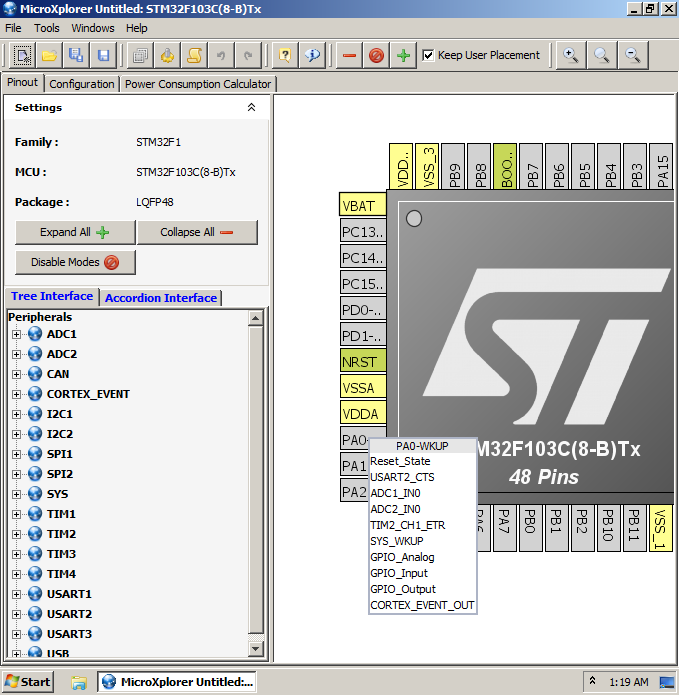
\includegraphics[width=250pt]{images/microxplorer}
			\end{center}
		\end{exampleblock}
	\end{frame}

	\section{TheEnd}
	\begin{frame}
		\frametitle{Sakalangkong Sadejenah}
		\begin{exampleblock}{}
			Butuh training atau development di Programming/Embedded-System/IoT?\\
			Code-Direct siap membantu. CP:
			\begin{itemize}
				\item Wahyu Anggoro: 0857-6944-2009
				\item Sangsaka Wira: 0858-9973-1884
			\end{itemize}
		\end{exampleblock}

		\begin{exampleblock}{}
			Butuh training atau development di 3D-Print/Welding/Engineering?\\
			FTITOS siap membantu. CP:
			\begin{itemize}
				\item Aurelia     : 0812-9676-6651
				\item Bagus Sadewa: 0822-6678-5789
			\end{itemize}
		\end{exampleblock}
	\end{frame}

\end{document}
